\chapter{Rotor FE}
\section{Beam Element FE Equation}
\subsection{Bernoulli-Euler Beam equation}
Assumptions used to derive the bernoulli-Euler beam equation are (Complete derivation in \cite{craig2006fundamentals}):
\begin{enumerate}
	\item Beam is bending in a plane, in this case in the y-direction, where the x-direction is along the length of the beam.
	\item The  neutral axis undergoes no deformation in the longitudinal direction.
	\item Cross sections remain plane and perpendicular to the nuetral axis.
	\item The material is linear-elastic.
	\item Stresses in the y and z direction are negligible compared to those in the x direction.
	\item Rotatory inertia may be neglected in moment equation.
	\item Mass density is constant at each cross section, so that each mass center is coincident with the centroid of that section.
\end{enumerate}
Using kinematics and assumptions 2 \& 3, the strain in the x direction may be related to the curvature of the beam, $\mu(x,t)$, and the distance from the neutral axis by
\begin{equation} \label{eq:curvature}
\epsilon=-\dfrac{y}{\mu}
\end{equation}
then, with assumption 4 \& 7 the relation from curvature to moment is
\begin{equation} \label{eq:curv_moment}
M(x,t)=\dfrac{EI}{\mu}
\end{equation}
\begin{figure}
	\centering
	\def\svgwidth{300pt}
	\import{figures/}{BeamFBD.pdf_tex}
	\caption{Free body diagram of a beam section in planar bending.}
	\label{fig:BeamFBD}
\end{figure}
where $ E $, Young's modulus, and $ I $, area moment of inertia are constant in cross sections. By using Newton's laws and the free body diagram of a single beam element, see Figure \ref{fig:BeamFBD}, the equations of motion are summarized as:
\begin{equation} \label{eq:Newton}
\sum{F_y}=\Delta m a_y \quad \textrm{\&} \quad \sum{M_G}=0
\end{equation}
Moment equation is represented as moments summarized at the center of mass, $ G $. The right hand side of moment equation of EOM \eqref{eq:Newton} is know to be null due to assumption 6. Applying Newton's equations \eqref{eq:Newton} to the FBD of Figure \ref{fig:BeamFBD} results in the force equation
\begin{equation} \label{eq:force_EOM}
F(x,t)-F(x+\Delta x,t)=\rho A\Delta x \frac{\partial^2 v}{\partial t^2}
\end{equation}
and moment equation
\begin{equation} \label{eq:moment_EOM}
-M(x,t) + M(x+\Delta x,t) + F(x,t)\left( \frac{-\Delta x}{2}\right)  + \left[-F(x+\Delta x,t)\right] \left(\frac{\Delta x}{2}\right) = 0
\end{equation}
Taking the limit of equations \eqref{eq:force_EOM} \& \eqref{eq:moment_EOM} as $ \Delta x \rightarrow 0 $ results in equations \eqref{eq:force_EOM_partial} \& \eqref{eq:moment_EOM_partial} respectively.
\begin{equation} \label{eq:force_EOM_partial}
\frac{\partial F}{\partial x}=-\rho A \frac{\partial^2 v}{\partial t^2}
\end{equation} 
\begin{equation} \label{eq:moment_EOM_partial}
\frac{\partial M}{\partial x} = F
\end{equation}
Assuming the beam slope, $ \frac{\partial v}{\partial x} $, remains relatively small, then linearized curvature of the beam is inversely proportional to $ \frac{\partial^2 v}{\partial x^2} $. Substituting this linearized curvature in \eqref{eq:curv_moment} produces
\begin{equation} \label{eq:moment_curvature_partial}
M(x,t)=EI\frac{\partial^2 v}{\partial x^2}
\end{equation}
Using linearized moment equation \eqref{eq:moment_curvature_partial}, combined with \eqref{eq:force_EOM_partial} \&  \eqref{eq:moment_EOM_partial} lends the Euler beam equation
\begin{equation} \label{eq:euler_beam_equation}
\frac{\partial^2}{\partial x^2} \left(EI\frac{\partial^2 v}{\partial x^2}\right) = -\rho A\frac{\partial^2 v}{\partial t^2}
\end{equation}
\begin{equation} \label{eq:Hooke's_Law}
T=k\delta
\end{equation}
\begin{equation} \label{eq:Potential_energy_gov}
\pi_p=\frac{1}{2}k(u_2 -u_1)^2-f_{1x} u_1-f_{2x}u_2
\end{equation}

This is the governing differential equation for transverse motion of a slender beam. This equation is not suitable for an application involving lengths that are not much greater than the width of the beam \cite{genta2007dynamics}.
\begin{figure}[h!]
	\centering
	% This file was created by matlab2tikz.
%
%The latest updates can be retrieved from
%  http://www.mathworks.com/matlabcentral/fileexchange/22022-matlab2tikz-matlab2tikz
%where you can also make suggestions and rate matlab2tikz.
%
\definecolor{mycolor1}{rgb}{0.92900,0.69400,0.12500}%
\definecolor{mycolor2}{rgb}{0.46600,0.67400,0.18800}%
\definecolor{mycolor3}{rgb}{0.63500,0.07800,0.18400}%
\definecolor{mycolor4}{rgb}{0.85000,0.32500,0.09800}%
\definecolor{mycolor5}{rgb}{0.49400,0.18400,0.55600}%
\definecolor{mycolor6}{rgb}{0.30100,0.74500,0.93300}%
%
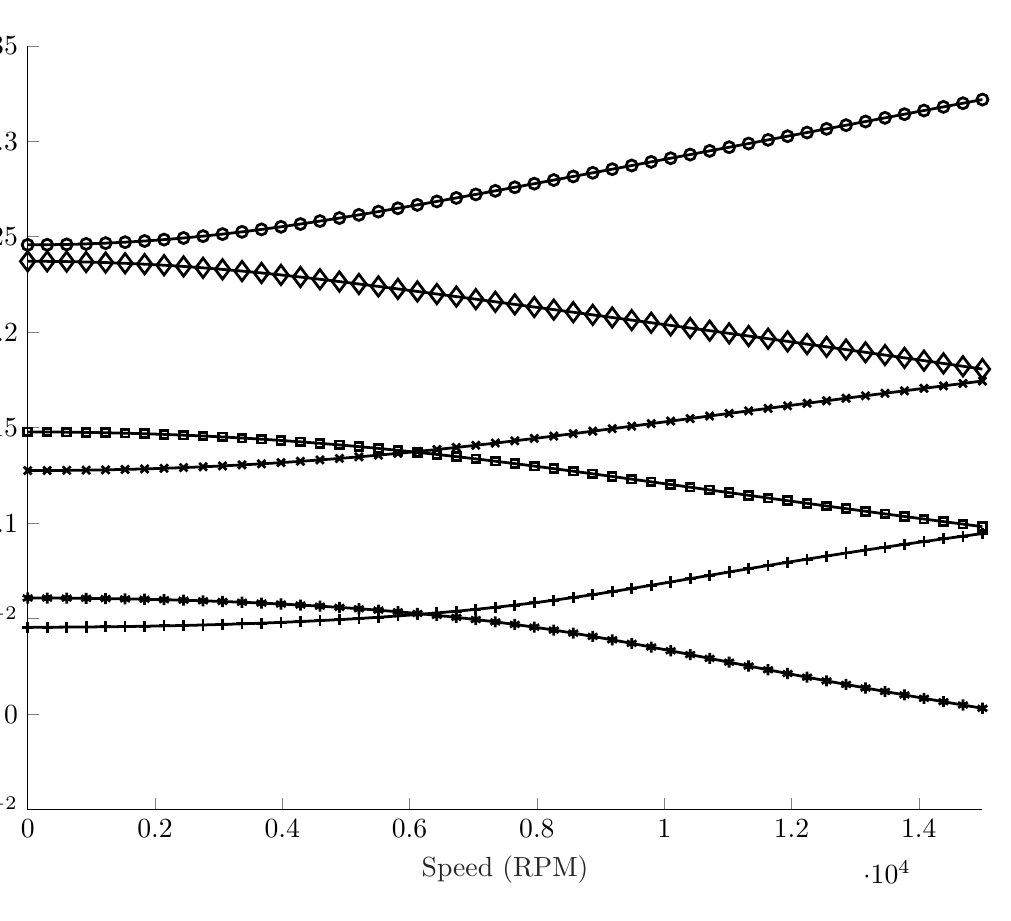
\begin{tikzpicture}[trim axis left, trim axis right]

\begin{axis}[%
width=\linewidth,
height=.8\linewidth,
%at={(0.758in,0.504in)},
scale only axis,
xmin=0,
xmax=15000,
xlabel style={font=\color{white!15!black}},
xlabel={Speed (RPM)},
ymin=-0.05,
ymax=0.35,
ylabel style={font=\color{white!15!black}},
ylabel={Damping Ratio},
axis background/.style={fill=white},
axis x line*=left,
axis y line*=left
]
\addplot [color=mycolor1, forget plot]
  table[row sep=crcr]{%
0	0.0455259517696042\\
306.122448979592	0.0455398894477022\\
612.244897959184	0.0455817707000235\\
918.367346938776	0.0456517987867038\\
1224.48979591837	0.045750317064802\\
1530.61224489796	0.0458778120029195\\
1836.73469387755	0.0460349203375184\\
2142.85714285714	0.0462224377991348\\
2448.97959183673	0.0464413291448113\\
2755.10204081633	0.0466927431602038\\
3061.22448979592	0.0469780263318186\\
3367.34693877551	0.0472987423545407\\
3673.4693877551	0.0476566931226369\\
3979.59183673469	0.0480539424214631\\
4285.71428571429	0.0484928421729271\\
4591.83673469388	0.0489760602263476\\
4897.95918367347	0.0495066088527385\\
5204.08163265306	0.0500878698507127\\
5510.20408163265	0.0507236163052227\\
5816.32653061224	0.0514180190364786\\
6122.44897959184	0.052175632606571\\
6428.57142857143	0.0530013438092034\\
6734.69387755102	0.053900263914818\\
7040.81632653061	0.0548775379250932\\
7346.9387755102	0.0559380421079406\\
7653.0612244898	0.0570859361875718\\
7959.18367346939	0.0583240816904186\\
8265.30612244898	0.0596533225031999\\
8571.42857142857	0.0610717568168187\\
8877.55102040816	0.0625741523836269\\
9183.67346938776	0.0641517268456452\\
9489.79591836735	0.0657924723046449\\
9795.91836734694	0.0674820503636735\\
10102.0408163265	0.0692050856138768\\
10408.1632653061	0.0709465401129494\\
10714.2857142857	0.0726928407940573\\
11020.4081632653	0.0744325817184057\\
11326.5306122449	0.0761567700268819\\
11632.6530612245	0.0778587347870482\\
11938.7755102041	0.0795338246730914\\
12244.8979591837	0.0811790304228755\\
12551.0204081633	0.0827926061106241\\
12857.1428571429	0.0843737399191389\\
13163.2653061224	0.0859222837485895\\
13469.387755102	0.0874385459075488\\
13775.5102040816	0.088923133912004\\
14081.6326530612	0.0903768417262804\\
14387.7551020408	0.0918005691920008\\
14693.8775510204	0.0931952660146588\\
15000	0.0945618929643459\\
};
\addplot [color=black, line width=1.0pt, mark size=2.0pt, mark=+, mark options={solid, black}, forget plot]
  table[row sep=crcr]{%
0	0.0455259517696042\\
306.122448979592	0.0455398894477022\\
612.244897959184	0.0455817707000235\\
918.367346938776	0.0456517987867038\\
1224.48979591837	0.045750317064802\\
1530.61224489796	0.0458778120029195\\
1836.73469387755	0.0460349203375184\\
2142.85714285714	0.0462224377991348\\
2448.97959183673	0.0464413291448113\\
2755.10204081633	0.0466927431602038\\
3061.22448979592	0.0469780263318186\\
3367.34693877551	0.0472987423545407\\
3673.4693877551	0.0476566931226369\\
3979.59183673469	0.0480539424214631\\
4285.71428571429	0.0484928421729271\\
4591.83673469388	0.0489760602263476\\
4897.95918367347	0.0495066088527385\\
5204.08163265306	0.0500878698507127\\
5510.20408163265	0.0507236163052227\\
5816.32653061224	0.0514180190364786\\
6122.44897959184	0.052175632606571\\
6428.57142857143	0.0530013438092034\\
6734.69387755102	0.053900263914818\\
7040.81632653061	0.0548775379250932\\
7346.9387755102	0.0559380421079406\\
7653.0612244898	0.0570859361875718\\
7959.18367346939	0.0583240816904186\\
8265.30612244898	0.0596533225031999\\
8571.42857142857	0.0610717568168187\\
8877.55102040816	0.0625741523836269\\
9183.67346938776	0.0641517268456452\\
9489.79591836735	0.0657924723046449\\
9795.91836734694	0.0674820503636735\\
10102.0408163265	0.0692050856138768\\
10408.1632653061	0.0709465401129494\\
10714.2857142857	0.0726928407940573\\
11020.4081632653	0.0744325817184057\\
11326.5306122449	0.0761567700268819\\
11632.6530612245	0.0778587347870482\\
11938.7755102041	0.0795338246730914\\
12244.8979591837	0.0811790304228755\\
12551.0204081633	0.0827926061106241\\
12857.1428571429	0.0843737399191389\\
13163.2653061224	0.0859222837485895\\
13469.387755102	0.0874385459075488\\
13775.5102040816	0.088923133912004\\
14081.6326530612	0.0903768417262804\\
14387.7551020408	0.0918005691920008\\
14693.8775510204	0.0931952660146588\\
15000	0.0945618929643459\\
};
\addplot [color=mycolor2, forget plot]
  table[row sep=crcr]{%
0	0.0608119830324956\\
306.122448979592	0.0607944160359\\
612.244897959184	0.0607416463848613\\
918.367346938776	0.0606534718391234\\
1224.48979591837	0.0605295495050181\\
1530.61224489796	0.0603693942743757\\
1836.73469387755	0.0601723710413995\\
2142.85714285714	0.0599376852802921\\
2448.97959183673	0.0596643750651212\\
2755.10204081633	0.0593512932698691\\
3061.22448979592	0.0589970956686628\\
3367.34693877551	0.0586002211059115\\
3673.4693877551	0.0581588702213003\\
3979.59183673469	0.0576709811413276\\
4285.71428571429	0.057134204503884\\
4591.83673469388	0.0565458735988659\\
4897.95918367347	0.055902977097797\\
5204.08163265306	0.0552021334864661\\
5510.20408163265	0.0544395688194617\\
5816.32653061224	0.0536111098369867\\
6122.44897959184	0.0527121974885157\\
6428.57142857143	0.0517379382124654\\
6734.69387755102	0.0506832116846406\\
7040.81632653061	0.0495428601118647\\
7346.9387755102	0.0483119902762683\\
7653.0612244898	0.0469864265537985\\
7959.18367346939	0.0455632818178439\\
8265.30612244898	0.0440416893022366\\
8571.42857142857	0.0424235268976443\\
8877.55102040816	0.0407140071598477\\
9183.67346938776	0.0389218981918823\\
9489.79591836735	0.0370592042387211\\
9795.91836734694	0.0351402722293824\\
10102.0408163265	0.033180497882503\\
10408.1632653061	0.0311949513215903\\
10714.2857142857	0.029197246521395\\
11020.4081632653	0.0271988353021962\\
11326.5306122449	0.0252087603735356\\
11632.6530612245	0.023233743714867\\
11938.7755102041	0.0212784865607901\\
12244.8979591837	0.0193460473901101\\
12551.0204081633	0.0174382202541397\\
12857.1428571429	0.0155558629373129\\
13163.2653061224	0.0136991686390495\\
13469.387755102	0.0118678734238633\\
13775.5102040816	0.0100614131929158\\
14081.6326530612	0.0082790375964813\\
14387.7551020408	0.00651988943441405\\
14693.8775510204	0.00478306267785321\\
15000	0.00306763985306097\\
};
\addplot [color=black, line width=1.0pt, mark size=2.0pt, mark=asterisk, mark options={solid, black}, forget plot]
  table[row sep=crcr]{%
0	0.0608119830324956\\
306.122448979592	0.0607944160359\\
612.244897959184	0.0607416463848613\\
918.367346938776	0.0606534718391234\\
1224.48979591837	0.0605295495050181\\
1530.61224489796	0.0603693942743757\\
1836.73469387755	0.0601723710413995\\
2142.85714285714	0.0599376852802921\\
2448.97959183673	0.0596643750651212\\
2755.10204081633	0.0593512932698691\\
3061.22448979592	0.0589970956686628\\
3367.34693877551	0.0586002211059115\\
3673.4693877551	0.0581588702213003\\
3979.59183673469	0.0576709811413276\\
4285.71428571429	0.057134204503884\\
4591.83673469388	0.0565458735988659\\
4897.95918367347	0.055902977097797\\
5204.08163265306	0.0552021334864661\\
5510.20408163265	0.0544395688194617\\
5816.32653061224	0.0536111098369867\\
6122.44897959184	0.0527121974885157\\
6428.57142857143	0.0517379382124654\\
6734.69387755102	0.0506832116846406\\
7040.81632653061	0.0495428601118647\\
7346.9387755102	0.0483119902762683\\
7653.0612244898	0.0469864265537985\\
7959.18367346939	0.0455632818178439\\
8265.30612244898	0.0440416893022366\\
8571.42857142857	0.0424235268976443\\
8877.55102040816	0.0407140071598477\\
9183.67346938776	0.0389218981918823\\
9489.79591836735	0.0370592042387211\\
9795.91836734694	0.0351402722293824\\
10102.0408163265	0.033180497882503\\
10408.1632653061	0.0311949513215903\\
10714.2857142857	0.029197246521395\\
11020.4081632653	0.0271988353021962\\
11326.5306122449	0.0252087603735356\\
11632.6530612245	0.023233743714867\\
11938.7755102041	0.0212784865607901\\
12244.8979591837	0.0193460473901101\\
12551.0204081633	0.0174382202541397\\
12857.1428571429	0.0155558629373129\\
13163.2653061224	0.0136991686390495\\
13469.387755102	0.0118678734238633\\
13775.5102040816	0.0100614131929158\\
14081.6326530612	0.0082790375964813\\
14387.7551020408	0.00651988943441405\\
14693.8775510204	0.00478306267785321\\
15000	0.00306763985306097\\
};
\addplot [color=mycolor3, forget plot]
  table[row sep=crcr]{%
0	0.127559830791334\\
306.122448979592	0.127583897780293\\
612.244897959184	0.127656140995403\\
918.367346938776	0.127776694968729\\
1224.48979591837	0.127945776611992\\
1530.61224489796	0.128163684224583\\
1836.73469387755	0.128430787680519\\
2142.85714285714	0.128747519512198\\
2448.97959183673	0.129114364071218\\
2755.10204081633	0.12953183401747\\
3061.22448979592	0.130000456208468\\
3367.34693877551	0.130520740573442\\
3673.4693877551	0.131093153173253\\
3979.59183673469	0.131718076786157\\
4285.71428571429	0.132395769526562\\
4591.83673469388	0.133126317419722\\
4897.95918367347	0.133909582515609\\
5204.08163265306	0.134745150851755\\
5510.20408163265	0.135632275539813\\
5816.32653061224	0.136569833413084\\
6122.44897959184	0.13755628241441\\
6428.57142857143	0.138589638151886\\
6734.69387755102	0.139667465527669\\
7040.81632653061	0.140786898023604\\
7346.9387755102	0.141944677886015\\
7653.0612244898	0.143137222927786\\
7959.18367346939	0.144360712596116\\
8265.30612244898	0.145611188743668\\
8571.42857142857	0.146884662665417\\
8877.55102040816	0.148177220024271\\
9183.67346938776	0.149485115423928\\
9489.79591836735	0.150804848886668\\
9795.91836734694	0.152133224948447\\
10102.0408163265	0.153467391280357\\
10408.1632653061	0.154804851322306\\
10714.2857142857	0.156143469017845\\
11020.4081632653	0.157481452044195\\
11326.5306122449	0.15881733125381\\
11632.6530612245	0.160149928616221\\
11938.7755102041	0.161478327951131\\
12244.8979591837	0.162801839095324\\
12551.0204081633	0.164119966830484\\
12857.1428571429	0.165432380987739\\
13163.2653061224	0.166738888957873\\
13469.387755102	0.168039409999641\\
13775.5102040816	0.169333956019727\\
14081.6326530612	0.170622611961482\\
14387.7551020408	0.171905519596836\\
14693.8775510204	0.173182864488186\\
15000	0.17445486802699\\
};
\addplot [color=black, line width=1.0pt, mark size=2.0pt, mark=x, mark options={solid, black}, forget plot]
  table[row sep=crcr]{%
0	0.127559830791334\\
306.122448979592	0.127583897780293\\
612.244897959184	0.127656140995403\\
918.367346938776	0.127776694968729\\
1224.48979591837	0.127945776611992\\
1530.61224489796	0.128163684224583\\
1836.73469387755	0.128430787680519\\
2142.85714285714	0.128747519512198\\
2448.97959183673	0.129114364071218\\
2755.10204081633	0.12953183401747\\
3061.22448979592	0.130000456208468\\
3367.34693877551	0.130520740573442\\
3673.4693877551	0.131093153173253\\
3979.59183673469	0.131718076786157\\
4285.71428571429	0.132395769526562\\
4591.83673469388	0.133126317419722\\
4897.95918367347	0.133909582515609\\
5204.08163265306	0.134745150851755\\
5510.20408163265	0.135632275539813\\
5816.32653061224	0.136569833413084\\
6122.44897959184	0.13755628241441\\
6428.57142857143	0.138589638151886\\
6734.69387755102	0.139667465527669\\
7040.81632653061	0.140786898023604\\
7346.9387755102	0.141944677886015\\
7653.0612244898	0.143137222927786\\
7959.18367346939	0.144360712596116\\
8265.30612244898	0.145611188743668\\
8571.42857142857	0.146884662665417\\
8877.55102040816	0.148177220024271\\
9183.67346938776	0.149485115423928\\
9489.79591836735	0.150804848886668\\
9795.91836734694	0.152133224948447\\
10102.0408163265	0.153467391280357\\
10408.1632653061	0.154804851322306\\
10714.2857142857	0.156143469017845\\
11020.4081632653	0.157481452044195\\
11326.5306122449	0.15881733125381\\
11632.6530612245	0.160149928616221\\
11938.7755102041	0.161478327951131\\
12244.8979591837	0.162801839095324\\
12551.0204081633	0.164119966830484\\
12857.1428571429	0.165432380987739\\
13163.2653061224	0.166738888957873\\
13469.387755102	0.168039409999641\\
13775.5102040816	0.169333956019727\\
14081.6326530612	0.170622611961482\\
14387.7551020408	0.171905519596836\\
14693.8775510204	0.173182864488186\\
15000	0.17445486802699\\
};
\addplot [color=mycolor4, forget plot]
  table[row sep=crcr]{%
0	0.147779939226167\\
306.122448979592	0.147754061840429\\
612.244897959184	0.147676393488211\\
918.367346938776	0.1475468096263\\
1224.48979591837	0.147365115596344\\
1530.61224489796	0.147131039413527\\
1836.73469387755	0.146844246438042\\
2142.85714285714	0.146504348896789\\
2448.97959183673	0.146110911339576\\
2755.10204081633	0.145663477098252\\
3061.22448979592	0.145161586397288\\
3367.34693877551	0.144604797656032\\
3673.4693877551	0.14399272010994\\
3979.59183673469	0.143325055348906\\
4285.71428571429	0.142601632198534\\
4591.83673469388	0.14182245731783\\
4897.95918367347	0.140987766456383\\
5204.08163265306	0.140098079436447\\
5510.20408163265	0.139154246864117\\
5816.32653061224	0.138157507650032\\
6122.44897959184	0.137109523847237\\
6428.57142857143	0.136012404882525\\
6734.69387755102	0.13486871768512\\
7040.81632653061	0.133681468182845\\
7346.9387755102	0.132454061142044\\
7653.0612244898	0.131190236110319\\
7959.18367346939	0.129893976449722\\
8265.30612244898	0.128569414622232\\
8571.42857142857	0.127220723281184\\
8877.55102040816	0.125852004655653\\
9183.67346938776	0.124467206434246\\
9489.79591836735	0.12307003280111\\
9795.91836734694	0.121663891086886\\
10102.0408163265	0.120251851687577\\
10408.1632653061	0.118836631197097\\
10714.2857142857	0.117420590575178\\
11020.4081632653	0.116005745653356\\
11326.5306122449	0.114593795445016\\
11632.6530612245	0.113186142712457\\
11938.7755102041	0.111783931348721\\
12244.8979591837	0.110388077615791\\
12551.0204081633	0.108999298350194\\
12857.1428571429	0.107618146446865\\
13163.2653061224	0.106245033962157\\
13469.387755102	0.104880256887352\\
13775.5102040816	0.103524015429139\\
14081.6326530612	0.102176433943101\\
14387.7551020408	0.10083757604726\\
14693.8775510204	0.0995074547860546\\
15000	0.0981860483060968\\
};
\addplot [color=black, line width=1.0pt, mark size=1.4pt, mark=square, mark options={solid, black}, forget plot]
  table[row sep=crcr]{%
0	0.147779939226167\\
306.122448979592	0.147754061840429\\
612.244897959184	0.147676393488211\\
918.367346938776	0.1475468096263\\
1224.48979591837	0.147365115596344\\
1530.61224489796	0.147131039413527\\
1836.73469387755	0.146844246438042\\
2142.85714285714	0.146504348896789\\
2448.97959183673	0.146110911339576\\
2755.10204081633	0.145663477098252\\
3061.22448979592	0.145161586397288\\
3367.34693877551	0.144604797656032\\
3673.4693877551	0.14399272010994\\
3979.59183673469	0.143325055348906\\
4285.71428571429	0.142601632198534\\
4591.83673469388	0.14182245731783\\
4897.95918367347	0.140987766456383\\
5204.08163265306	0.140098079436447\\
5510.20408163265	0.139154246864117\\
5816.32653061224	0.138157507650032\\
6122.44897959184	0.137109523847237\\
6428.57142857143	0.136012404882525\\
6734.69387755102	0.13486871768512\\
7040.81632653061	0.133681468182845\\
7346.9387755102	0.132454061142044\\
7653.0612244898	0.131190236110319\\
7959.18367346939	0.129893976449722\\
8265.30612244898	0.128569414622232\\
8571.42857142857	0.127220723281184\\
8877.55102040816	0.125852004655653\\
9183.67346938776	0.124467206434246\\
9489.79591836735	0.12307003280111\\
9795.91836734694	0.121663891086886\\
10102.0408163265	0.120251851687577\\
10408.1632653061	0.118836631197097\\
10714.2857142857	0.117420590575178\\
11020.4081632653	0.116005745653356\\
11326.5306122449	0.114593795445016\\
11632.6530612245	0.113186142712457\\
11938.7755102041	0.111783931348721\\
12244.8979591837	0.110388077615791\\
12551.0204081633	0.108999298350194\\
12857.1428571429	0.107618146446865\\
13163.2653061224	0.106245033962157\\
13469.387755102	0.104880256887352\\
13775.5102040816	0.103524015429139\\
14081.6326530612	0.102176433943101\\
14387.7551020408	0.10083757604726\\
14693.8775510204	0.0995074547860546\\
15000	0.0981860483060968\\
};
\addplot [color=mycolor5, forget plot]
  table[row sep=crcr]{%
0	0.245752400547887\\
306.122448979592	0.245808259454918\\
612.244897959184	0.245975966665432\\
918.367346938776	0.246255893615347\\
1224.48979591837	0.246648588797306\\
1530.61224489796	0.247154666234691\\
1836.73469387755	0.247774649337821\\
2142.85714285714	0.248508746617158\\
2448.97959183673	0.249356594127014\\
2755.10204081633	0.250316952298878\\
3061.22448979592	0.251387412304587\\
3367.34693877551	0.252564141234411\\
3673.4693877551	0.253841749115933\\
3979.59183673469	0.255213311738633\\
4285.71428571429	0.256670595737527\\
4591.83673469388	0.258204434415531\\
4897.95918367347	0.259805234904081\\
5204.08163265306	0.261463476293955\\
5510.20408163265	0.26317015199565\\
5816.32653061224	0.264917093041429\\
6122.44897959184	0.266697139737562\\
6428.57142857143	0.268504192371662\\
6734.69387755102	0.270333179288176\\
7040.81632653061	0.272179946629548\\
7346.9387755102	0.274041141489721\\
7653.0612244898	0.275914074095581\\
7959.18367346939	0.277796600137654\\
8265.30612244898	0.279687001367395\\
8571.42857142857	0.281583906083014\\
8877.55102040816	0.283486204785573\\
9183.67346938776	0.285392984131724\\
9489.79591836735	0.287303500769427\\
9795.91836734694	0.289217120823588\\
10102.0408163265	0.291133297528893\\
10408.1632653061	0.29305156285068\\
10714.2857142857	0.294971489561984\\
11020.4081632653	0.296892697819963\\
11326.5306122449	0.298814831264036\\
11632.6530612245	0.300737560996988\\
11938.7755102041	0.302660571622347\\
12244.8979591837	0.304583566639965\\
12551.0204081633	0.306506258423394\\
12857.1428571429	0.308428369830448\\
13163.2653061224	0.310349629108224\\
13469.387755102	0.312269780402744\\
13775.5102040816	0.314188564682791\\
14081.6326530612	0.31610573432394\\
14387.7551020408	0.318021052582538\\
14693.8775510204	0.319934282838545\\
15000	0.321845200283609\\
};
\addplot [color=black, line width=1.0pt, mark size=2.0pt, mark=o, mark options={solid, black}, forget plot]
  table[row sep=crcr]{%
0	0.245752400547887\\
306.122448979592	0.245808259454918\\
612.244897959184	0.245975966665432\\
918.367346938776	0.246255893615347\\
1224.48979591837	0.246648588797306\\
1530.61224489796	0.247154666234691\\
1836.73469387755	0.247774649337821\\
2142.85714285714	0.248508746617158\\
2448.97959183673	0.249356594127014\\
2755.10204081633	0.250316952298878\\
3061.22448979592	0.251387412304587\\
3367.34693877551	0.252564141234411\\
3673.4693877551	0.253841749115933\\
3979.59183673469	0.255213311738633\\
4285.71428571429	0.256670595737527\\
4591.83673469388	0.258204434415531\\
4897.95918367347	0.259805234904081\\
5204.08163265306	0.261463476293955\\
5510.20408163265	0.26317015199565\\
5816.32653061224	0.264917093041429\\
6122.44897959184	0.266697139737562\\
6428.57142857143	0.268504192371662\\
6734.69387755102	0.270333179288176\\
7040.81632653061	0.272179946629548\\
7346.9387755102	0.274041141489721\\
7653.0612244898	0.275914074095581\\
7959.18367346939	0.277796600137654\\
8265.30612244898	0.279687001367395\\
8571.42857142857	0.281583906083014\\
8877.55102040816	0.283486204785573\\
9183.67346938776	0.285392984131724\\
9489.79591836735	0.287303500769427\\
9795.91836734694	0.289217120823588\\
10102.0408163265	0.291133297528893\\
10408.1632653061	0.29305156285068\\
10714.2857142857	0.294971489561984\\
11020.4081632653	0.296892697819963\\
11326.5306122449	0.298814831264036\\
11632.6530612245	0.300737560996988\\
11938.7755102041	0.302660571622347\\
12244.8979591837	0.304583566639965\\
12551.0204081633	0.306506258423394\\
12857.1428571429	0.308428369830448\\
13163.2653061224	0.310349629108224\\
13469.387755102	0.312269780402744\\
13775.5102040816	0.314188564682791\\
14081.6326530612	0.31610573432394\\
14387.7551020408	0.318021052582538\\
14693.8775510204	0.319934282838545\\
15000	0.321845200283609\\
};
\addplot [color=mycolor6, forget plot]
  table[row sep=crcr]{%
0	0.237155367657664\\
306.122448979592	0.237113889396312\\
612.244897959184	0.236989253994067\\
918.367346938776	0.236780963416423\\
1224.48979591837	0.236488214558676\\
1530.61224489796	0.236110052978996\\
1836.73469387755	0.235645532382073\\
2142.85714285714	0.235093904450786\\
2448.97959183673	0.234454916765749\\
2755.10204081633	0.233729111113687\\
3061.22448979592	0.232918098120593\\
3367.34693877551	0.232024851770824\\
3673.4693877551	0.231053849730632\\
3979.59183673469	0.23001102743828\\
4285.71428571429	0.228903599179782\\
4591.83673469388	0.227739672663695\\
4897.95918367347	0.226527754791685\\
5204.08163265306	0.225276249409699\\
5510.20408163265	0.223993040060018\\
5816.32653061224	0.222685136743276\\
6122.44897959184	0.221358532117927\\
6428.57142857143	0.220018144441701\\
6734.69387755102	0.218667852694617\\
7040.81632653061	0.217310609036963\\
7346.9387755102	0.2159485675011\\
7653.0612244898	0.214583207917028\\
7959.18367346939	0.213215489073515\\
8265.30612244898	0.211845942965566\\
8571.42857142857	0.210474774577839\\
8877.55102040816	0.209101963421761\\
9183.67346938776	0.207727294119886\\
9489.79591836735	0.206350435319102\\
9795.91836734694	0.204970969917883\\
10102.0408163265	0.203588431198561\\
10408.1632653061	0.202202319296708\\
10714.2857142857	0.200812133913941\\
11020.4081632653	0.199417380797688\\
11326.5306122449	0.198017567292871\\
11632.6530612245	0.196612244327301\\
11938.7755102041	0.195200979914302\\
12244.8979591837	0.193783377164586\\
12551.0204081633	0.192359078855455\\
12857.1428571429	0.190927767632552\\
13163.2653061224	0.189489156415569\\
13469.387755102	0.188043000043622\\
13775.5102040816	0.18658909568458\\
14081.6326530612	0.185127272596811\\
14387.7551020408	0.183657386226241\\
14693.8775510204	0.182179340802864\\
15000	0.180693061330394\\
};
\addplot [color=black, line width=1.0pt, mark size=3.5pt, mark=diamond, mark options={solid, black}, forget plot]
  table[row sep=crcr]{%
0	0.237155367657664\\
306.122448979592	0.237113889396312\\
612.244897959184	0.236989253994067\\
918.367346938776	0.236780963416423\\
1224.48979591837	0.236488214558676\\
1530.61224489796	0.236110052978996\\
1836.73469387755	0.235645532382073\\
2142.85714285714	0.235093904450786\\
2448.97959183673	0.234454916765749\\
2755.10204081633	0.233729111113687\\
3061.22448979592	0.232918098120593\\
3367.34693877551	0.232024851770824\\
3673.4693877551	0.231053849730632\\
3979.59183673469	0.23001102743828\\
4285.71428571429	0.228903599179782\\
4591.83673469388	0.227739672663695\\
4897.95918367347	0.226527754791685\\
5204.08163265306	0.225276249409699\\
5510.20408163265	0.223993040060018\\
5816.32653061224	0.222685136743276\\
6122.44897959184	0.221358532117927\\
6428.57142857143	0.220018144441701\\
6734.69387755102	0.218667852694617\\
7040.81632653061	0.217310609036963\\
7346.9387755102	0.2159485675011\\
7653.0612244898	0.214583207917028\\
7959.18367346939	0.213215489073515\\
8265.30612244898	0.211845942965566\\
8571.42857142857	0.210474774577839\\
8877.55102040816	0.209101963421761\\
9183.67346938776	0.207727294119886\\
9489.79591836735	0.206350435319102\\
9795.91836734694	0.204970969917883\\
10102.0408163265	0.203588431198561\\
10408.1632653061	0.202202319296708\\
10714.2857142857	0.200812133913941\\
11020.4081632653	0.199417380797688\\
11326.5306122449	0.198017567292871\\
11632.6530612245	0.196612244327301\\
11938.7755102041	0.195200979914302\\
12244.8979591837	0.193783377164586\\
12551.0204081633	0.192359078855455\\
12857.1428571429	0.190927767632552\\
13163.2653061224	0.189489156415569\\
13469.387755102	0.188043000043622\\
13775.5102040816	0.18658909568458\\
14081.6326530612	0.185127272596811\\
14387.7551020408	0.183657386226241\\
14693.8775510204	0.182179340802864\\
15000	0.180693061330394\\
};
\end{axis}
\end{tikzpicture}%
	\caption{Damping Figure.}
	\label{fig:Damp_Fig}
\end{figure}
\begin{equation} \label{eq:FEGoverning}
u(x,y,z,t)=N(x,y,z)q(t)
\end{equation}